\documentclass{article}

\usepackage[utf8]{inputenc}
\usepackage[hidelinks]{hyperref}
\usepackage{enumitem}
\usepackage{amsmath}
\usepackage{amsfonts}
\usepackage{tikz}

\usetikzlibrary{positioning}
\setlist[itemize]{after=\vspace{.5\baselineskip}}

\begin{document}
\author{Herman Bergwerf}
\title{QEDb: a database to create computer checked proofs with a focus on applied sciences}
\maketitle

\begin{abstract}
This document  outlines a database for storing simple algebraic proofs from various fields in applied sciences.  The goal of this database is to provide a proof reference resource that is detailed enough for computer programs to find the exact steps used in each proof derivation. This allows a computer system to create a personalized version of a proof, and to show its steps with a very high level of detail if requested by the user. The primary goal of this database is not to find new proofs. It is designed with little prior knowledge about computer aided proof checking. The design and implementation are from a programmer perspective. The database and its underlying rule based engine are implemented in the Dart programming language.\footnote{The code can be found at \url{https://github.com/qedb}} Implementation details are not discussed in this paper, instead it focuses on the conceptual design and some related questions that are not directly relevant for the implementation.
\end{abstract}
\section{Overview}
Writing down a proof starts with an initial mathematical expression. This expression is manipulated according to a list of steps that will produce the final expression. All intermediate expressions are considered to be equivalent. There are three methods available to manipulate the expression. Each method will be discussed in section \ref{section:expression-manipulation}.
\begin{itemize}
\item Argument rearrangement
\item Rule substitution
\item Condition substitution
\end{itemize}

Proofs are a sequence of such manipulations and show in a fundamental way that the final expression can be formed from the initial one by applying all intermediary steps. There are some specific cases when the result of a manipulation can be checked, but not reconstructed from the previous expression. This is sufficient for the purpose of this database. A proof can be re-used in other proofs, which provides a way to vastly simplify the building of new proofs. \par
To provide an interface where proofs can be constructed easily, a set of algorithms is used that can compare the difference between two expressions with all possible manipulations in order to find a sequence of manipulations that satisfies the difference. \par
Although an important goal is a high level of internal consistency and mathematical correctness, this cannot be guaranteed in all cases. In a number of cases mathematical integrity is sacrificed for simplicity and usability. This means that the checking algorithms cannot validate everything. It is possible to enter incorrect rules into the system (e.g. $2\rightarrow1$), to start proofs with a bad expression (e.g. $2=1$), or to substitute variables with expressions that have a different class (e.g. while time in classical mechanics is usually intended as a real scalar, there is no mechanism that restricts the user from substituting it with a vector). The order in which manipulations are done can also affect the outcome, more about this in section \ref{section:substitution-loophole}.

\section{Expressions}
Mathematical expressions are the cornerstone of this database. These expressions follow a very simple tree like structure that reminds of an Abstract Syntax Tree. Expressions are composed of functions and integers. A function is a node with an associated ID and a number of arguments. The argument count is fixed for each function ID, and is specified globally. From this a tree can be constructed like in figure \ref{fig:ast}. Symbols, such as $\pi$, can be expressed as functions with no arguments.

\begin{figure}
\centering
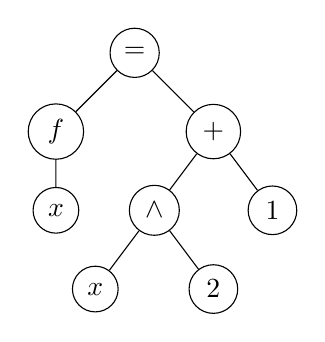
\begin{tikzpicture} [every node/.style={circle,draw},
  level 1/.style={level distance=10mm, sibling distance=20mm},
  level 2/.style={level distance=10mm, sibling distance=15mm}]
\node {$=$}
  child { node {$f$}
    child { node {$x$} }
  }
  child { node {$+$}
    child { node {$\wedge$}
      child { node {$x$} }
      child { node {$2$} }
    }
    child { node {$1$} }
  };
\end{tikzpicture}
\caption{Tree representation for the expression $f(x)=x^2+1$} \label{fig:ast}
\end{figure}

Functions can also be generic, meaning they can be replaced with an arbitrary expression. Generic functions play an important role in the formation of general rules. To avoid too much complexity, generics do not have any additional constraints. A variable such as $x$ in $f(x)=x^2+1$ can be expressed as a  generic function with no arguments. Now $x$ can be substituted with any expression, not just a scalar. Therefore the integrity of proofs also depends on the proof author.

\subsection{Why not use classes for generic functions?}
It would be possible to expand the integrity of substitutions of generic functions by including some classification system. For example, we could define $x$ in the previous example to be a real number, e.g. $x\in\mathbb{R}^1$. The reason such a mechanism is avoided is (1) to simplify the overall implementation, and (2) because determining the class of a function quickly becomes very hard. For example, to know that $1+\vec{u}\cdot\vec{v}$ reduces to $\mathbb{R}^1$ would require the proof checker to have (vector) algebra knowledge built-in while in fact the goal is partially to avoid as much built-in assumptions as possible. The absence of such a class system could in part be resolved by conditions. More about this is described in section \ref{section:conditions}.

\subsection{Expression manipulation}
\label{section:expression-manipulation}
Expression manipulation happens in two ways: rearrangement and substitution (either with rules or conditions). The manipulation can take place at any point in the expression tree.

\subsubsection{Rearrangement}
Rearrangement is the first type of manipulation that can be applied to expressions. It is a combination of the commutative\footnote{$f(a,\,b)\rightarrow f(b,\,a)$ where $f$ is the operator} and associative\footnote{$f(f(a,\,b),\,c)\rightarrow f(a,\,f(b,\,c))$ and $f(f(a,\,b),\,f(c,\,d))\rightarrow f(a,\,f(f(b,\,c),\,d))$} property of some binary operators (in particular addition and multiplication). A function can be defined to be rearrangeable, meaning that they have these two properties (i.e. the order of operations does not matter). Rearranging the children then means changing the expression tree (applying the operators in a different order), but keeping the same children as illustrated in figure \ref{fig:rearrange}. Instead of using fundamental rules to apply such manipulation, a custom algorithm can resolve rearrangements. This is done in order to avoid dealing with the vast number of substitutions that would result from such a common manipulation.

\begin{figure}
\centering
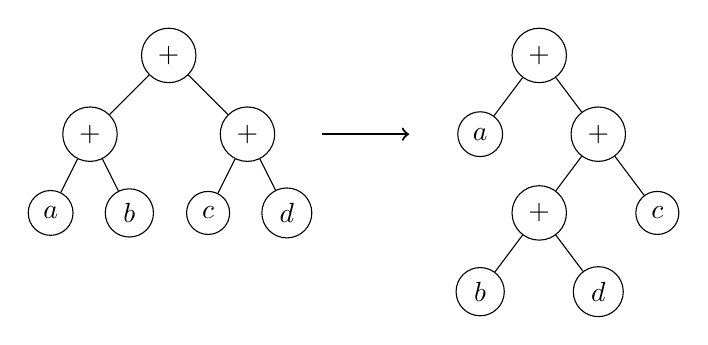
\begin{tikzpicture} [every node/.style={circle,draw}]

\tikzstyle{level 1}=[level distance=10mm, sibling distance=20mm]
\tikzstyle{level 2}=[level distance=10mm, sibling distance=10mm]
\node [left=2cm] {$+$}
  child { node {$+$}
    child { node {$a$} }
    child { node {$b$} }
  }
  child { node {$+$}
    child { node {$c$} }
    child { node {$d$} }
  };

\tikzstyle{level 1}=[level distance=10mm, sibling distance=15mm]
\tikzstyle{level 2}=[level distance=10mm, sibling distance=15mm]
\node [right=2cm] {$+$}
  child { node {$a$} }
  child { node {$+$}
    child { node {$+$}
      child { node {$b$} }
      child { node {$d$} }
    }
    child { node {$c$} }
  };
\draw [->, thick] (-.4,-1) to (.7,-1);
\end{tikzpicture}
\caption{Rearrangement from $(a+b)+(c+d)$ into $a+((b+d)+c)$} \label{fig:rearrange}
\end{figure}

\pagebreak
One possible sequence of five substitutions that would be required for the rearrangement shown in figure \ref{fig:rearrange} is as follows (only the fundamental properties may be used):
\begin{enumerate}
\item $(a+b)+(c+d)$
\item $a+((b+c)+d)$ which is a fundamental property
\item $a+((c+b)+d)$ by using $x+y\rightarrow y+x$
\item $a+(c+(b+d))$ by using $(x+y)+z\rightarrow x+(y+z)$
\item $a+((b+d)+c)$ by using $x+y\rightarrow y+x$
\end{enumerate}

\subsubsection{Substitution}
\label{section:substitution}
Substitution is the second type of manipulation that can be applied to expressions. Substitutions are executed using rules or conditions. Their role will become clear later. A substitution is applied at a certain point in the target expression tree, lets call this the substitution point. It also requires an equality between two expressions as input; a \emph{left} and \emph{right} expression. The left expression must match the expression at the substitution point, which will then be replaced with the right expression. Each generic functions in the left expression will be mapped to the expression at the same point in the target expression\footnote{This is sometimes called unification}. Naturally, a specific generic function can only be mapped to one expression for the left expression to match. This mapping is then substituted in the right expression. The expression at the substitution position is replaced with the resulting expression. This process is illustrated in figure \ref{fig:substitution}. 

\begin{figure}
\centering

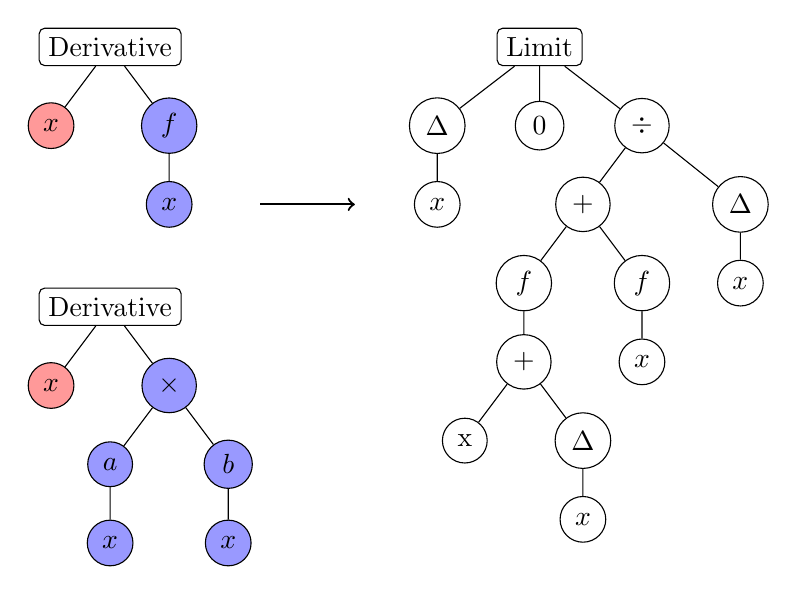
\begin{tikzpicture} [every node/.style={circle,draw}]
\tikzstyle{level 1}=[level distance=10mm, sibling distance=15mm]
\tikzstyle{level 2}=[level distance=10mm, sibling distance=10mm]
\node [left=2cm, rectangle, rounded corners=.2em] (diff) {Derivative}
  child { node [fill=red!40] {$x$} }
  child { node [fill=blue!40] {$f$}
    child { node [fill=blue!40] {$x$} }
  };

\tikzstyle{level 1}=[level distance=10mm, sibling distance=13mm]
\tikzstyle{level 2}=[level distance=10mm, sibling distance=15mm]
\node [right=2cm, rectangle, rounded corners=.2em] {Limit}
  child { node {$\Delta$}
    child { node {$x$} }
  }
  child { node {0} }
  child { node {$\div$}
    child { node {$+$}
      child { node {$f$}
        child { node {$+$}
          child { node {x} }
          child { node {$\Delta$} child { node {$x$} } }
        }
      }
      child { node {$f$} child { node {$x$} } }
    }
    child [sibling distance=25mm] { node {$\Delta$} child { node {$x$} } }
  };
\draw [->, thick] (-1,-2) -- (.2,-2);

\tikzstyle{level 1}=[level distance=10mm, sibling distance=15mm]
\node [rectangle, rounded corners=.2em, below=8em of diff] {Derivative}
child { node [fill=red!40] {$x$} }
child { node [fill=blue!40] {$\times$}
  child { node [fill=blue!40] {$a$}
    child { node [fill=blue!40] {$x$} }
  }
  child { node [fill=blue!40] {$b$}
    child { node [fill=blue!40] {$x$} }
  }
};
\end{tikzpicture}

\vspace{2em}

\begin{center}
  \def\arraystretch{1.5}
  \setlength{\tabcolsep}{1em}
  \begin{tabular}{ c|c }
    Generic function & Mapped to \\
    \hline
    $x$ & $x$ \\ 
    $f(x)$ & $a(x)b(x)$ \\
  \end{tabular}
\end{center}

\vspace{1em}
\begin{align} \frac{\partial}{\partial x}a(x)b(x)
\end{align}
\begin{align} \frac{\partial}{\partial x}f(x)=\lim_{\Delta x\to0}\frac{f(x+\Delta x)-f(x)}{\Delta x}
\end{align}
\begin{align} \lim_{\Delta x\to0}\frac{a(x+\Delta x)b(x+\Delta x)-a(x)b(x)}{\Delta x}
\end{align}
\vspace{1em}

\caption{Eq. 2 is substituted in Eq. 1, resulting in Eq. 3. The trees again show how the program sees the expression. The mapping of $f(x)$ is achieved by substituting $f(x)=a(x)b(x)$ into the right expression} \label{fig:substitution}
\end{figure}

\newpage

\subsubsection{Substitution order can matter}
\label{section:substitution-loophole}
When function dependencies are not explicitly pointed out in expressions, different substitution sequences can lead to different results. In some cases this can even lead to a discrepancy, in particular when a generic function is substituted with an expression that again contains this generic function. To illustrate this, lets look at an example similar to the one in figure \ref{fig:substitution}.

\begin{equation} b=2x
\end{equation}
\begin{equation} g(x)=a(x)b
\end{equation}
\begin{equation} \frac{\partial}{\partial x}g(x)=\lim_{\Delta x\to0}\frac{g(x+\Delta x)-g(x)}{\Delta x}
\end{equation}
\begin{equation} \frac{\partial}{\partial x}a(x)b=\lim_{\Delta x\to0}\frac{a(x+\Delta x)b-a(x)b}{\Delta x}
\end{equation}
\begin{equation} \frac{\partial}{\partial x}a(x)2x\neq\lim_{\Delta x\to0}\frac{a(x+\Delta x)2x-a(x)2x}{\Delta x}
\end{equation}
\begin{equation} \frac{\partial}{\partial x}a(x)2x=\lim_{\Delta x\to0}\frac{a(x+\Delta x)2(x+\Delta x)-a(x)2x}{\Delta x}
\end{equation}

\vspace{1em}

When applying the definition of the derivative to a function $g(x)$, we get Eq. 6. Now lets substitute the definition we have for $g(x)$ in Eq. 5. Note that the result is exactly the same as first substituting $g(x)=a(x)b$ in the derivative and then applying the limit definition. If we now substitute the definition of $b$ to get Eq. 8, we have a serious problem. Since $b$ was defined without function argument, the delta expression is not substituted in $2x$. Meanwhile, if we first substitute $g(x)$ \emph{and} $b$ in the derivative and \emph{then} substitute the limit definition, we do get the expected result. To prevent this, it would be sufficient to define $b(x)=2x$ instead of $b=2x$. In this case that seems pretty trivial, however other cases may arise where the dependencies are not always obvious ahead of time, or are not explicitly written down. For example, in classical mechanics it is quite common to write $\vec{a}$ instead of $\vec{a}(t)$, even when the acceleration depends on the time point. Obviously the initial rule set is the weak link here, and the database has no means of verifying the fundamental rules it is given. \par
It is possible to add some constraints to substitutions that restrict this, and at least prevent the case described here. To do this the substitution algorithm has to discard any substitution where a generic function is mapped to an expression that depends on any other function but the first argument of the generic function. This means the generic function can have 1 argument at most (this issue does not apply to generic functions with no arguments). For this to work all functions in the database have to be symbols or pure functions. This implies that all functions are either defined with no arguments, and can depend on any other function in the database, or \emph{only} depend on the arguments given. Such a constraint is enforced in QEDb.

\section{Rules}
A rule is an equation of a left and right expression, and can be used for substitutions. QEDb has a global set of rules that can be used in all contexts. Experiments with subject bounded rules have been done, however this approach did not reveal any significant advantages. Fundamental rules can be entered into the database, and from these more rules can be derived by first creating a proof, and then adding a rule based on a proof. The global rule-set has to be kept at a reasonable size to allow relatively quick difference resolving (section \ref{section:difference-resolving}).

\subsection{Semi-generic rules}
Often, rules have to be semi-generic. For example Newtons second law, $F=ma$, describes a general rule for all kinds of different forces. However this rule cannot be substituted when a different symbol is used for $F$ (e.g. $F_g$) because $F$, $m$ and $a$ are not generic. Making them generic would cause obvious problems. One way to solve this issue is to use a non-generic, single argument function for each context-dependent symbol. The argument of these function indicates the context. This way the rule can be created using a new generic symbol $ctx$: $F(ctx)\rightarrow m\cdot a(ctx)$. In this case subscript might look more familiar: $F_{ctx}\rightarrow m\cdot a_{ctx}$. For the gravitational force a new non-generic symbol $g$ can be defined and used with the semi-generic rule to get: $F_g\rightarrow m\cdot a_g$. 

\subsection{Conditions}
\label{section:conditions}
Creating a proof in QEDb is tedious work compared to writing out the proof on paper, every single assumption and algebraic operation has to be defined, proven and substituted. But the limitations of generic functions in creating general rules become very obvious when looking at the following simple case.

\begin{align} \frac{\partial g}{\partial x}=0
\end{align}
\begin{align}
\frac{\partial (g\cdot f)}{\partial x}
&= \frac{\partial g}{\partial x}\cdot f+g\cdot\frac{\partial f}{\partial x}\\
&= 0\cdot f+g\cdot\frac{\partial f}{\partial x}\\
&= g\cdot\frac{\partial f}{\partial x}
\end{align}

\newpage

The fact that you can move everything out of the derivative that is constant with respect to $x$ is something that is often taken for granted, but since this database does not have any built-in mathematics knowledge rules like this one have to be provide as well. There is one big inconvenience though, since Eq. 13 relies on Eq. 10, it has to be proven separately for every single case using the steps shown here (introducing Eq. 10 as a generic rule would obviously not be possible, then all possible derivatives would suddenly be equal to zero). To solve this inconvenience rules can have conditions. Using conditions this case can be expressed as:

\begin{equation} \frac{\partial (g\cdot f)}{\partial x}=g\cdot\frac{\partial f}{\partial x}
\quad\textrm{for}\quad
\frac{\partial g}{\partial x}=0
\end{equation}

When substituting the rule, another rule has to be referenced that satisfies the conditions (or multiple when there are multiple rules). There are some built-in conditions for special cases. For example the derivative of an integer is always zero, and the database can handle this automatically because it is not possible to create a rule for this since there is no way to limit a generic symbol to integers. \par
Conditions are limited to rule like structures; it has to be possible to look them up in the rule-set. Conditions are added by substituting them at some point in the proof. This means that while creating a proof, any arbitrary equation that is not in the rule-set can be substituted as a condition.

\subsection{Avoiding conflicts within the rule set}
To prevent conflicting or ambiguous rules, it is necessary to check any new rules against all existing rules. So when a new rule is submitted the database will check if a rule already exist that directly proves the new rule, or if the new rule directly proves any existing rules. If this is the case the new rule is rejected.

\section{Proofs}
The final piece of the puzzle are proofs. Proofs have been mentioned before, but there are a few things left to say about them. Proofs can be started with any arbitrary expression. If the proof is the manipulation of one side of an equation, for example the derivation of centripetal acceleration by working out the second derivative of the position vector, then it is possible to start with $a_c$ and end up at $v^2/r$ by applying a range of manipulations. However when an equation has to be solved for one variable, for example when solving $2x+10=5$ for $x$, it is necessary to start with the entire equation as first expression. The equals operator is just another 2-argument function in the database. Just like before, fundamental rules can be added to rearrange this expression such as $a+b=c\rightarrow a=c-b$. \par
A few basic functions, including addition, subtraction and multiplication, will be automatically evaluated after each step. Other functions are left unevaluated and are, by convention, part of the algebraic solution. Evaluation is done when all arguments are integers, and should always produce an integer. So for example, applying the rule $a^ba^c\rightarrow a^{b+c}$ to $a^2a^3$ will produce $a^5$ as resulting expression.

\subsection{Automatic difference resolving}
\label{section:difference-resolving}
QEDb can compare two expressions and find a tree of manipulations that satisfy their difference. This is achieved by recursively comparing both expressions, their arguments, etc., and matching them against the rule-set. Before looking for rules, an algorithm will determine whether the difference is due to a rearrangement. Rearrangements can be nested, so when comparing $a+(b+(c\cdot e))$ with $(e\cdot c)+b+a$, the algorithm will determine that two rearrangements took place. This automatic resolving help to create an intuitive interface for building proofs.

\section{Similar software}
There are many projects that implement a computer aided proof checker, and some have used it to build some sort of database. When I started out building this database I was not aware of most projects that have been done in the past (in part because I did not know what exactly to look for). The design of QEDb is not directly inspired by other projects, although the concepts that are used are pretty generic.

\subsection{ProofWiki}
The ProofWiki is basically a very well organized MediaWiki containing articles for a wide range of proofs. The proofs presented in the ProofWiki go far beyond what QEDb can do. In fact QEDb is mostly limited to analytic and algebraic proofs.

\subsection{MetaMath}
MetaMath employs a similar proof checking system as QEDb to construct a huge database of theorems that prove fundamental mathematical properties starting with ideas from set theory.

\end{document}
